% ==================================================
% CHAPTER 1: Introduction %
% ==================================================

\chapter{Introduction}
\label{chap:intro}
% Edit count: Lia - 0, Brigitte - 0

% Miscellaneous intros
%The Large Hadron Collider (LHC) and the ATLAS experiment were designed to search for a Higgs boson~\cite{atlas_letter_of_intent_1992}
%The primary goal in building the Large Hadron Collider (LHC) and the ATLAS experiment was to search for a Higgs boson
%Studying particle detectors is interesting because of the interplay between the physics of what is to be studied with the detector and the physics of how the detector works. 
%Particle detectors intertwine physics concepts at multiple scales since their use requires understanding both the physics of how they work and the physics of what they are meant to study. 
%The details of how a particle detector works intertwine with the physics it is meant to study. Especially in a collaboration as large as ATLAS. 
%Small-strip thin gap chambers (sTGCs) for the ATLAS experiment at CERN 
%The questions proposed in the first recorded physics case for the Large Hadron Collider (LHC) are still only partially answered~\cite{brianti_large_1984}. it is clear there is still more to study at the LHC if the study of the %standard model is to continue. 
%The High-Lumnosity Large Hadron Collider (HL-LHC) project was approved to combat the plateau in statistial gain of recording particle collisions at the LHC at CERN~\cite{apollinari_high-luminosity_2017}. 
%The questions proposed in the first recorded physics case for the Large Hadron Collider (LHC) are still only 
%If the study of particle physics is to continue, studying the Higgs boson 

\section{Introduction}

THIS IS REALLY ROUGH. BASED ON ALESSANDRO'S IDEA OF SHOWING THE FULL INTRO OVERVIEW THEN DIVING INTO ALL THE NECESSARY DETAILS.

The High-Lumnosity Large Hadron Collider (HL-LHC) project was approved to combat the plateau in statistial gain of recording particle collisions at the LHC at CERN~\cite{apollinari_high-luminosity_2017}. Being the most energetic particle accelerator, the LHC still offers unique physics opportunities for studying the Higgs and electroweak sectors of the standard model; if the study of the standard model is to continue, the LHC must go on. The HL-LHC upgrade aims to \textcolor{red}{increase the luminosity of the LHC by up to a factor of 10 in the next 10 years, namely by increasing the proton-proton collision rate}. Naturally, various sub-systems of the experiments used to capture the outcomes of the collisions will require upgrades to handle higher collision rates and background radiation rates than they were designed for. 

The ATLAS experiment is one of the LHC's general-purpose particle detector arrays. The largest upgrade the ATLAS experiment will undergo is the replacement of the small wheels of the muon spectrometer with the so-called New Small Wheels (NSWs). Two different detector technologies will be installed: micromegas, and small-strip thin gap chambers (or sTGCs). In this work, the dataset used to correct for the internal alignment of sTGC components is validated with characterization data collected on the sTGCs using cosmic muons. How the internal alignment fits into the overall alignment system is also detailed. 

Information necessary to understand the ATLAS detector, the NSW upgrade, sTGCs and the NSW alignment system are presented. In chapter 2, the details of how cosmic muon data was collected are presented. In chapter 3, I explain one way cosmic muon data can be used for alignment. BLAH BLAH BLAH. 

\section{Background}

\subsection{The Large Hadron Collider}
\textcolor{red}{cite later!}

The LHC is an accelerator \SI{27}{\kilo\meter} in circumference and located TILDA\SI{100}{\meter} underground near Geneva, Switzerland~\cite{evans_lhc_2008}. It has two beam pipes with counter-circulating bunches of protons (usually) which are made to collide in the center of one of four major experiments. For example, the ATLAS experiment is a general-purpose detector designed to capture the outcome of the collisions. In the previous run of ATLAS (run 2) protons were collided with a center of mass energy of \SI{13}{\tera\electronvolt} - which is the energy frontier in particle physics. 

There are two main branches of study that can be pursued with the LHC and ATLAS. First, properties predicted by the standard model (SM) of particle physics can be measured. Otherwise, physicists can search for evidence of processes predicted by theories beyond the standard model. Both the SM measurement and search analyses are based on estimating the number of times a given process occurs. In this way, the number of proton-proton interactions created by the LHC directly affects the statistics available to do measurements or searches using the ATLAS experiment.

Predicting the number of proton-proton interactions requires defining a metric called luminosity. It is the number of particles an accelerator can send through a given area per unit time. It is calculated from the measurable quantities in equation~\ref{eqn:inst_lum}.

\begin{equation}
\mathcal{L} = \frac{f N_{1} N_{2} }{4 \pi \sigma_{x} \sigma_{y}}
\label{eqn:inst_lum}
\end{equation}

In equation~\ref{eqn:inst_lum}, $f$ is the frequency of the bunch crossings, $N_{1}$ and $N_{2}$ are the number of protons in each bunch, and $\sigma_{x}$ and $\sigma_{y}$ are the RMS of the spatial distributions of the bunch; therefore, luminosity comes from how the accelerator is run. Multiplying the luminosity by the cross section of a given process gives the expected rate for that process.

Integrating the \textit{instantaneous} luminosity over a period of data collection gives the integrated luminosity,

\begin{equation}
L = \int \mathcal{L} \left( t \right) \,dt
\label{eqn:int_lum}
\end{equation}

measured as an inverse cross section and related to the total number of collisions. In this way, the luminosity is the link between the accelerator and the statistical power of measurements to be made with the data collected. 

% This is not how you fb-1
So far, the LHC provided \SI{30}{\per\fempto\barn} of collisions in run 1 and \SI{150}{\per\fempto\barn} of collisions in run 2, as shown in figure~\ref{fig:hl-lhc}. The HL-LHC upgrade was accepted because without increasing the luminosity of the LHC roughly tenfold, running the accelerator will not provide significant statistical gain on measurements and its systems will need repair and replacement to operate past TILDA 2020. The energy accessible at the LHC provides irreplaceable ability to study Higgs and electroweak sector physics worldwide [ cite Physics at a High-Luminosity LHC with ATLAS ?], so the European Strategy for Particle Physics made it a priority "to fully exploit the physics potential of the LHC" with "a major luminosity upgrade." [Cite (from HLLHC TDR: https://council.web.cern.ch/en/EuropeanStrategy/ESParticlePhysics.html] The goal is for the LHC to provide \SI{3000}{\per\fempto\barn} of collisions in the 12 years following the upgrade. Success hinges on a combination of technological advances and upgrades being worked on now~\cite{hl_lhc_tdr}.


\begin{figure}
    \centering
    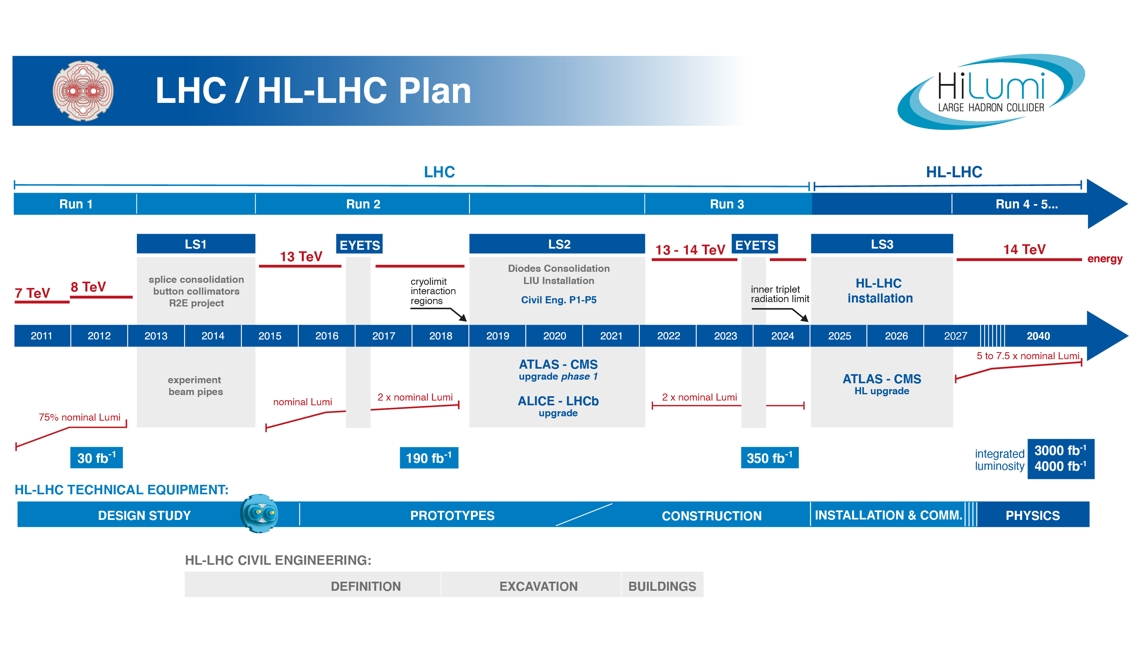
\includegraphics[width = \textwidth]{figures/HL-LHC-updated-January-2021_small.jpg}
    \caption{LHC/HL-LHC plan~\cite{hl-lhc_plan_picture_website}. The integrated luminosity collected and projected for each run of the LHC is shown in red below the timeline and the center of mass energy of the collisions is shown in red above the timeline. "LS" stands for "long shutdown" and indicates periods where the accelerator was not operating, but upgrades of the LHC and experiments were being installed. This timeline was last updated in January, 2021, and reflects changes in the schedule due to the ongoing pandemic. }
    \label{fig:hl-lhc}
\end{figure}







%The estimated number of interactions of a given type per bunch crossing is given by equation~\ref{eqn:num_interactions}.
%\begin{equation}
%\mu = \sigma \delta t\mathcal{L}
%\label{eqn:num_interactions}
%\end{equation}

So luminosity is key to 

It is mostly used to collide protons at a center-of-mass energy of \SI{13}{\tera\electronvolt} - which is the energy frontier of particle physics. Two main particle detector arrays, including the ATLAS experiment, are used to capture the outcome of the collisions. 



The energies accessible by the accelerator make it unique infrastructure with which to study processes of the standard model of particle physics and search for new phenomenon beyond the standard model. Considerable progress has been made towards answering the questions originally used to motivate the construction of the LHC, but many remain unanswered or only partially answered~\cite{brianti_large_1984}. Therefore, the continued use and maintenance of the accelerator 
- pp collisions
- 13 TeV
- luminosity - it is increasing

\subsection{The ATLAS experiment}

\subsection{The ATLAS muon spectrometer}
The outermost detector subsystem of ATLAS is the muon spectrometer since muons, being minimum ionizing particles, are not stopped by the calorimeters.

The muon spectrometer is the outermost layer of the ATLAS detector, since only muons (and neutrinos) can pass through the calorimeters. For muons that are ejected towards the end-caps of ATLAS, their trajectory is bent by the magentic field and their position recorded by three successive wheels of muon detectors. With each wheel providing the position of the muon along its trajectory and knowledge of the magentic field, the momentum of the muon generated in the collision can be reconstructed. 

\subsection{Motivation for replacing the NSW}
Currently, the small wheel is made of thin-gap chambers, whi22ch record hits. They have the known problem that particles generated in the material of the end-cap toroid magnet that hit the small wheel cannot be distinguished from muons from the interaction point. For example, in figure~\ref{fig:nsw_track_triggering}, all three tracks would be triggered on.

\begin{figure}
    \centering
    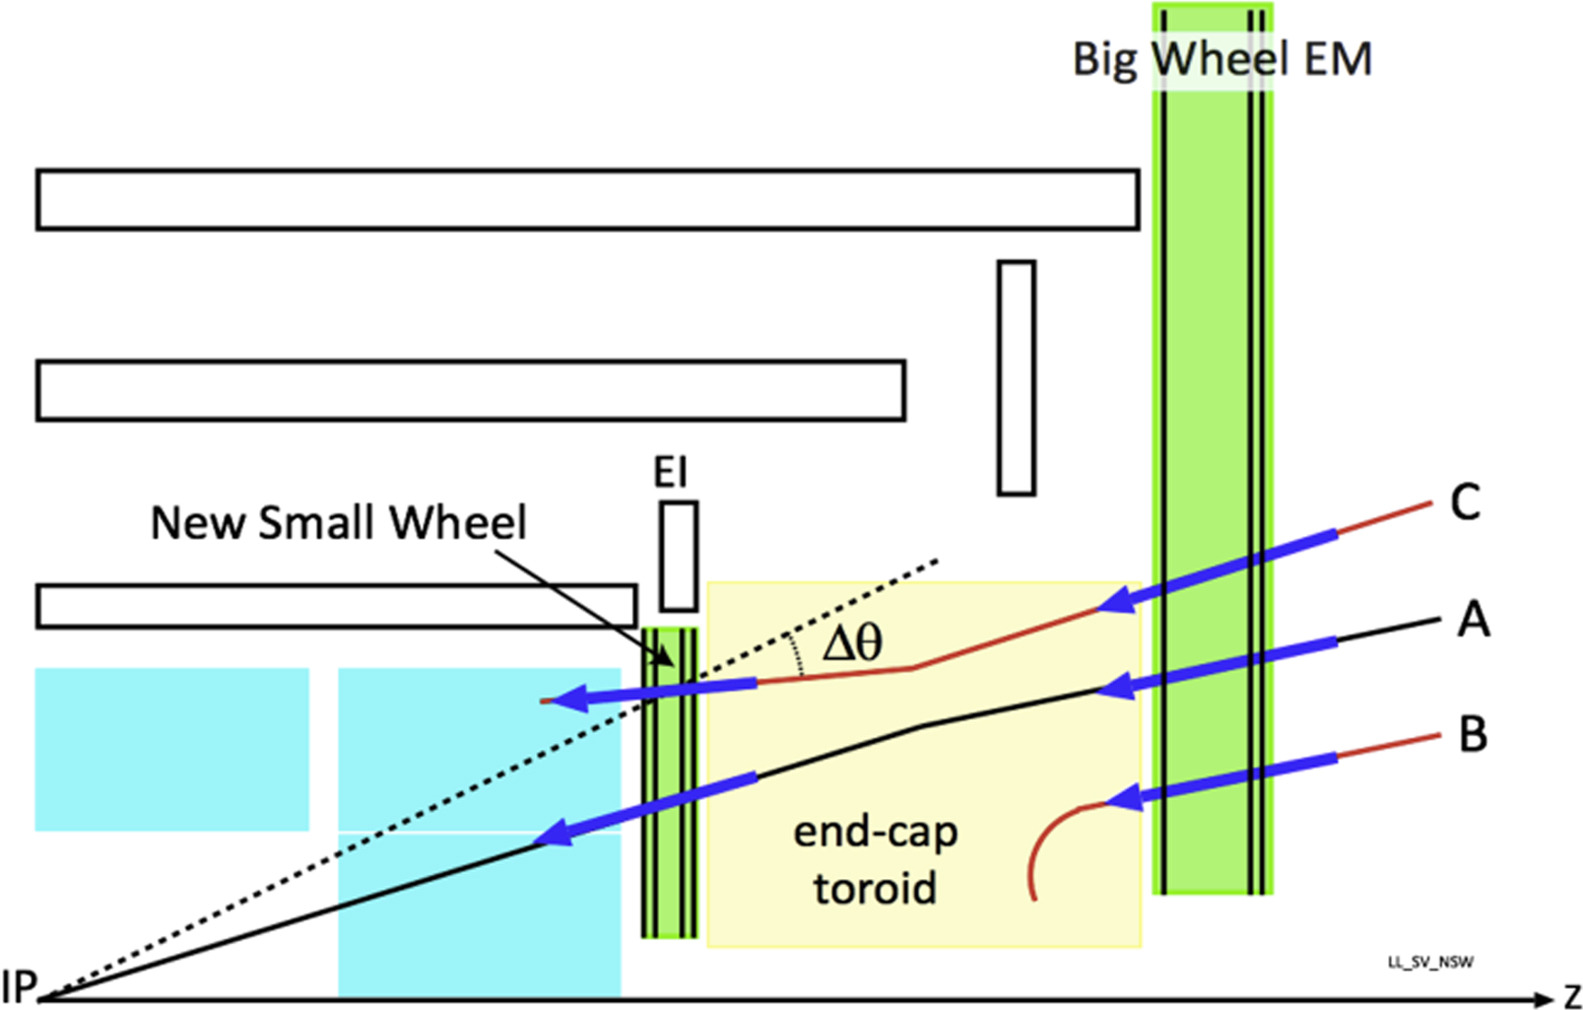
\includegraphics[width = 0.9\textwidth]{figures/perez-codina_NSW_tracks.jpg}
    \caption{A schematic of a quarter cross section of the ATLAS detector, with the collision/interaction point (IP) in the bottom left corner. Three possible tracks are labelled. Ideally, track A would be triggered upon while track B and C discarded. With the small wheel, only the big wheel provides the trigger so all three tracks would be recorded. With the new small wheel, only track A would be recorded.}
    \label{fig:nsw_track_triggering}
\end{figure}



